\documentclass[tikz,border=15pt]{standalone}
\usepackage{amsmath}
\usetikzlibrary{backgrounds} 

\begin{document}
	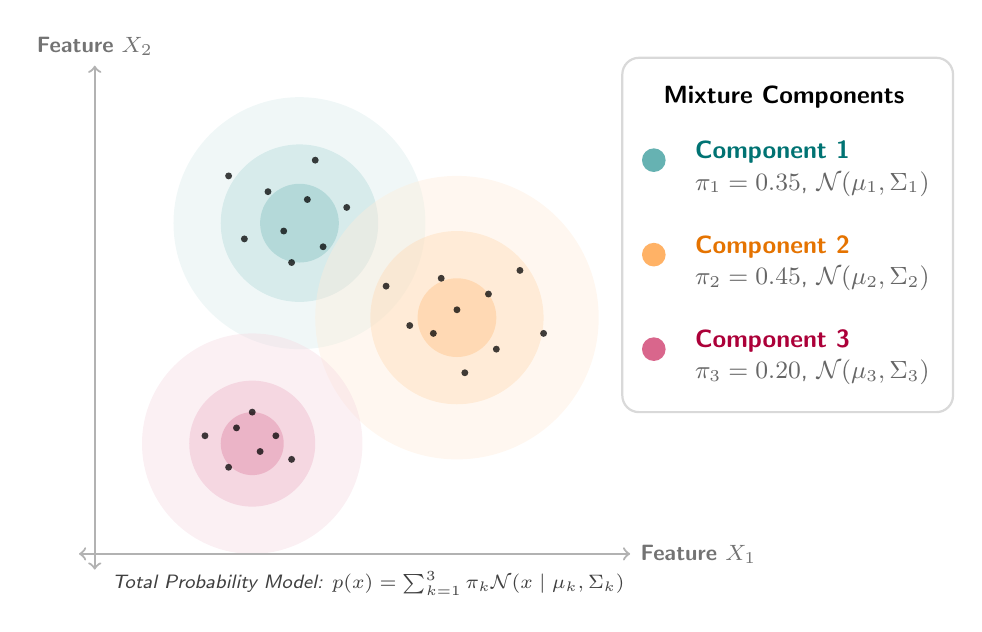
\begin{tikzpicture}[
		font=\sffamily,
		% Styling for individual generated data points
		datapoint/.style={circle, fill=black, inner sep=0pt, minimum size=2.5pt, opacity=0.75},
		% Typography enhancements (Fixed missing /.style suffix)
		labelstyle/.style={align=left, font=\sffamily\small},
		titlestyle/.style={font=\sffamily\bfseries\small}
		]
		
		% =========================================================================
		% CLUSTER 1: Teal Sub-population (Top-Left)
		% =========================================================================
		\begin{scope}[shift={(0,1.8)}]
			\fill[teal!15, opacity=0.4] (0,0) circle (1.6cm);
			\fill[teal!30, opacity=0.4] (0,0) circle (1.0cm);
			\fill[teal!50, opacity=0.4] (0,0) circle (0.5cm);
			
			\node[datapoint] at (0.1, 0.3) {};
			\node[datapoint] at (-0.2, -0.1) {};
			\node[datapoint] at (-0.4, 0.4) {};
			\node[datapoint] at (0.3, -0.3) {};
			\node[datapoint] at (-0.1, -0.5) {};
			\node[datapoint] at (0.6, 0.2) {};
			\node[datapoint] at (-0.7, -0.2) {};
			\node[datapoint] at (0.2, 0.8) {};
			\node[datapoint] at (-0.9, 0.6) {};
		\end{scope}
		
		% =========================================================================
		% CLUSTER 2: Orange Sub-population (Center-Right, Overlapping)
		% =========================================================================
		\begin{scope}[shift={(2.0,0.6)}]
			\fill[orange!15, opacity=0.4] (0,0) circle (1.8cm);
			\fill[orange!30, opacity=0.4] (0,0) circle (1.1cm);
			\fill[orange!50, opacity=0.4] (0,0) circle (0.5cm);
			
			\node[datapoint] at (0.0, 0.1) {};
			\node[datapoint] at (-0.3, -0.2) {};
			\node[datapoint] at (0.4, 0.3) {};
			\node[datapoint] at (-0.2, 0.5) {};
			\node[datapoint] at (0.5, -0.4) {};
			\node[datapoint] at (-0.6, -0.1) {};
			\node[datapoint] at (0.1, -0.7) {};
			\node[datapoint] at (0.8, 0.6) {};
			\node[datapoint] at (-0.9, 0.4) {};
			\node[datapoint] at (1.1, -0.2) {};
		\end{scope}
		
		% =========================================================================
		% CLUSTER 3: Purple Sub-population (Bottom-Left)
		% =========================================================================
		\begin{scope}[shift={(-0.6,-1.0)}]
			\fill[purple!15, opacity=0.4] (0,0) circle (1.4cm);
			\fill[purple!30, opacity=0.4] (0,0) circle (0.8cm);
			\fill[purple!50, opacity=0.4] (0,0) circle (0.4cm);
			
			\node[datapoint] at (0.1, -0.1) {};
			\node[datapoint] at (-0.2, 0.2) {};
			\node[datapoint] at (0.3, 0.1) {};
			\node[datapoint] at (-0.3, -0.3) {};
			\node[datapoint] at (0.0, 0.4) {};
			\node[datapoint] at (0.5, -0.2) {};
			\node[datapoint] at (-0.6, 0.1) {};
		\end{scope}
		
		% =========================================================================
		% LEGEND (SHIFTS & BOUNDS PERFECTLY BALANCED AND ALIGNED)
		% =========================================================================
		\begin{scope}[shift={(4.5, 2.5)}]
			% Header Text
			\node[titlestyle, anchor=west] at (0, 0.9) {Mixture Components};
			
			% Component 1 Elements
			\fill[teal!60] (0, 0.1) circle (0.15cm);
			\node[teal!90!black, titlestyle, anchor=west] at (0.4, 0.2) {Component 1};
			\node[gray!80!black, labelstyle, anchor=west] at (0.4, -0.2) {$\pi_1 = 0.35$, $\mathcal{N}(\mu_1, \Sigma_1)$};
			
			% Component 2 Elements
			\fill[orange!60] (0, -1.1) circle (0.15cm);
			\node[orange!90!black, titlestyle, anchor=west] at (0.4, -1.0) {Component 2};
			\node[gray!80!black, labelstyle, anchor=west] at (0.4, -1.4) {$\pi_2 = 0.45$, $\mathcal{N}(\mu_2, \Sigma_2)$};
			
			% Component 3 Elements
			\fill[purple!60] (0, -2.3) circle (0.15cm);
			\node[purple!90!black, titlestyle, anchor=west] at (0.4, -2.2) {Component 3};
			\node[gray!80!black, labelstyle, anchor=west] at (0.4, -2.6) {$\pi_3 = 0.20$, $\mathcal{N}(\mu_3, \Sigma_3)$};
			
			% Safe Background Border Container (Sized symmetrically around the text bounds)
			\begin{scope}[on background layer]
				\draw[gray!30, fill=white, rounded corners=6pt, line width=0.8pt] (-0.4, 1.4) rectangle (3.8, -3.1);
			\end{scope}
		\end{scope}
		
		% =========================================================================
		% AXES AND GLOBAL LABELS
		% =========================================================================
		\draw[<->, thick, gray!60] (-2.6,-2.6) -- (-2.6,3.8) node[above, text=gray!90!black, font=\sffamily\footnotesize\bfseries] {Feature $X_2$};
		\draw[<->, thick, gray!60] (-2.8,-2.4) -- (4.2,-2.4) node[right, text=gray!90!black, font=\sffamily\footnotesize\bfseries] {Feature $X_1$};
		
		\node[anchor=north west, text=gray!50!black, font=\sffamily\scriptsize\itshape] at (-2.5,-2.5) 
		{Total Probability Model: $p(x) = \sum_{k=1}^3 \pi_k \mathcal{N}(x \mid \mu_k, \Sigma_k)$};
		
	\end{tikzpicture}
\end{document}
